\chapter{Sun flare detection algorithm}

Before starting to write the main solar flare detection algorithm a first program was developed in which the location of the sun was known and we knew when the solar flare had taken place.

Try algorithm knowing the location of the source, sun. Show first distribution of VTEC thtough the day (vill), then for the specific moment in time


\section{Key elements}

\subsection{Correlation}

explain, formulas, references, etc

explain R and compare to show the computation is correct

\subsection{Moment of the flare}

explicar buscar pico por hill climbing o algo asi usando la grafica de la distribucion. Al encontrar un momento exacto en el que centrarnos empezar a estudiar ahi





\section{Brute force approach}

explicar que es para entender que debemos hacer

\subsection{Pseudocode}

primero pseudocodigo, explicar for each dec for each ra


\begin{algorithm}
	\caption{My algorithm}\label{euclid}
	\begin{algorithmic}[1]
		\Procedure{MyProcedure}{}
		\State $\textit{stringlen} \gets \text{length of }\textit{string}$
		\State $i \gets \textit{patlen}$
		\BState \emph{top}:
		\If {$i > \textit{stringlen}$} \Return false
		\EndIf
		\State $j \gets \textit{patlen}$
		\BState \emph{loop}:
		\If {$\textit{string}(i) = \textit{path}(j)$}
		\State $j \gets j-1$.
		\State $i \gets i-1$.
		\State \textbf{goto} \emph{loop}.
		\State \textbf{close};
		\EndIf
		\State $i \gets i+\max(\textit{delta}_1(\textit{string}(i)),\textit{delta}_2(j))$.
		\State \textbf{goto} \emph{top}.
		\EndProcedure
	\end{algorithmic}
\end{algorithm}

entonces explicar aqui lo de los polos, in a first approach to this in which to visually see ourselves the differences between possible Sun positions we obtained a plot for each possibility (figure \ref{fig:poles}), we could see this happening:

\begin{figure}[!htb]
	\begin{subfigure}[b]{0.5\textwidth}
		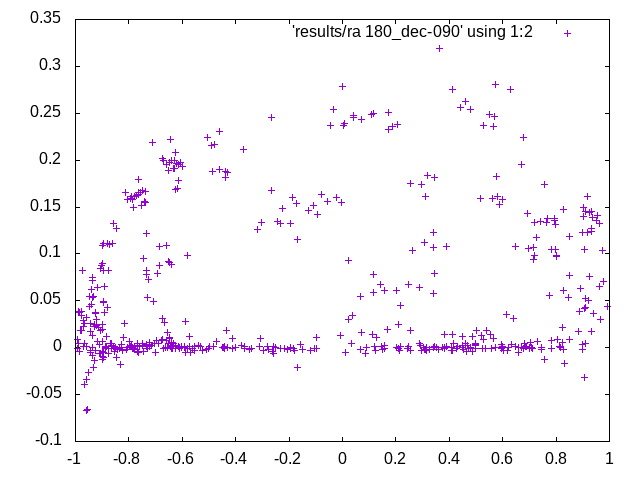
\includegraphics[width=\linewidth]{images/ch4/ra180_dec-090.png}
		\caption{ra180 and dec-090}
	\end{subfigure}
	\hfill
	\begin{subfigure}[b]{0.5\textwidth}
		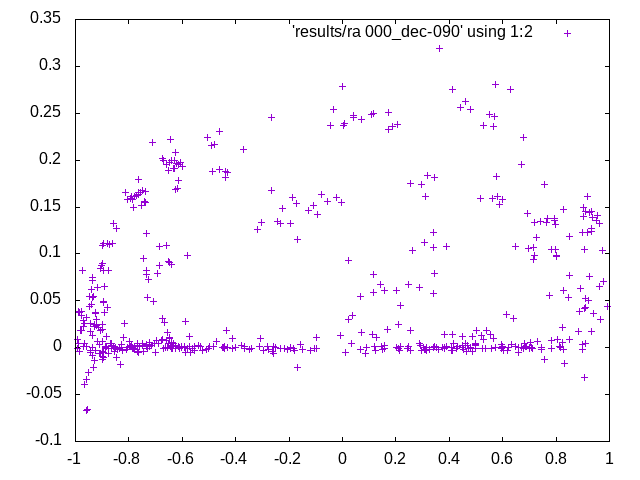
\includegraphics[width=\linewidth]{images/ch4/ra000_dec-090.png}
		\caption{ra000 and dec-090}
	\end{subfigure}
	\caption{dasdasdasda}
	\label{fig:poles}
\end{figure}


\subsection{Linking C++ and Fortran}

explicar aqui que la logica se hace con c++ y la computacion numerica con Fortran

\begin{lstlisting}[language=Python, caption=Python example]
import numpy as np

def incmatrix(genl1,genl2):
m = len(genl1)
n = len(genl2)
M = None #to become the incidence matrix
VT = np.zeros((n*m,1), int)  #dummy variable

#compute the bitwise xor matrix
M1 = bitxormatrix(genl1)
M2 = np.triu(bitxormatrix(genl2),1) 

for i in range(m-1):
for j in range(i+1, m):
[r,c] = np.where(M2 == M1[i,j])
for k in range(len(r)):
VT[(i)*n + r[k]] = 1;
VT[(i)*n + c[k]] = 1;
VT[(j)*n + r[k]] = 1;
VT[(j)*n + c[k]] = 1;

if M is None:
M = np.copy(VT)
else:
M = np.concatenate((M, VT), 1)

VT = np.zeros((n*m,1), int)

return M
\end{lstlisting}